% !TeX root = ../main.tex
% Copyright (c) 2026 Tyler Bignell
% Licensed under the MIT License - see LICENSE file for details

%%%%%%%%%%%%%%%%%%%%%%%%%%%%%%%%%%%%%%%%%%%%%%%%%%%%%%%%%%%
% FRONT MATTER
%%%%%%%%%%%%%%%%%%%%%%%%%%%%%%%%%%%%%%%%%%%%%%%%%%%%%%%%%%%
\begin{abstract} % Can \input abstract optionally
    \metaAbstract
\end{abstract}
\newpage

\tableofcontents
\newpage

\phantomsection % Allows TOC to link to todo list
\ifthenelse{\equal{\metaShowTodo}{true}}{%
	\addcontentsline{toc}{section}{Todo list}}{} % Creates TOC entry if metadata true
\listoftodos % Can be turned off in metadata

\phantomsection % Allows TOC to link to list of figures
\addcontentsline{toc}{section}{List of Figures} % Creates TOC entry
\listoffigures

\phantomsection % Allows TOC to link to list of tables
\addcontentsline{toc}{section}{List of Tables} % Creates TOC entry
\listoftables
\newpage

%%%%%%%%%%%%%%%%%%%%%%%%%%%%%%%%%%%%%%%%%%%%%%%%%%%%%%%%%%%
% CONDITIONALS
%%%%%%%%%%%%%%%%%%%%%%%%%%%%%%%%%%%%%%%%%%%%%%%%%%%%%%%%%%%
\section{Conditionals}

\subsection{\texttt{xifthen}}
The \texttt{xifthen} package extends \LaTeX's conditional logic with \texttt{\textbackslash ifthenelse} and \texttt{\textbackslash isempty}. It is used throughout this template to conditionally load packages and apply settings based on the metadata macros defined at the top of \texttt{main.tex}. It produces no visible output on its own.

% Example: check if metaPartners is empty
\ifthenelse{\equal{\metaPartners}{}}{
    \textit{No partners defined (default).}
}{
    \textit{Partners are defined.}
}

%%%%%%%%%%%%%%%%%%%%%%%%%%%%%%%%%%%%%%%%%%%%%%%%%%%%%%%%%%%
% COLORS
%%%%%%%%%%%%%%%%%%%%%%%%%%%%%%%%%%%%%%%%%%%%%%%%%%%%%%%%%%%
\section{Colors}

\subsection{\texttt{xcolor}}
The \texttt{xcolor} package provides extended color support. The template defines \texttt{facultycolour} as the primary brand color, automatically selected based on \texttt{\textbackslash metaFaculty} and \texttt{\textbackslash metaFacultyColour} in the metadata. It is used throughout headings, boxes, and rules.

\begin{table}[H]
	\centering
	\caption{Faculty colour and tints.}
	\label{tab:colors}
	\begin{tabular}{@{}lll@{}}
		\toprule
		Color Name & Hex & Preview \\
		\midrule
		\texttt{facultycolour} & 100\% tint & \textcolor{white}{\colorbox{facultycolour}{\quad\quad\quad}} \\
		\texttt{facultycolour!70} & 70\% tint & \textcolor{white}{\colorbox{facultycolour!70}{\quad\quad\quad}} \\
		\texttt{facultycolour!40} & 40\% tint & \colorbox{facultycolour!40}{\quad\quad\quad} \\
		\bottomrule
	\end{tabular}
\end{table}

Inline color: \textcolor{facultycolour}{This text is in the brand colour.}

%%%%%%%%%%%%%%%%%%%%%%%%%%%%%%%%%%%%%%%%%%%%%%%%%%%%%%%%%%%
% PAGE GEOMETRY
%%%%%%%%%%%%%%%%%%%%%%%%%%%%%%%%%%%%%%%%%%%%%%%%%%%%%%%%%%%
\section{Page Geometry}

\subsection{\texttt{geometry}}
The \texttt{geometry} package sets the page margins. This template uses 2.54\,cm (1 inch) margins on all sides with \texttt{headheight=14.9pt} to accommodate the header. These are set in \texttt{main.tex} and produce no visible output here.

\subsection{\texttt{setspace}}
The \texttt{setspace} package controls line spacing. The template supports \texttt{single}, \texttt{onehalf}, and \texttt{double} spacing, set via \texttt{\textbackslash metaLineSpacing} in the metadata. The current document uses \texttt{\metaLineSpacing} spacing.

%%%%%%%%%%%%%%%%%%%%%%%%%%%%%%%%%%%%%%%%%%%%%%%%%%%%%%%%%%%
% ENCODING & LANGUAGE
%%%%%%%%%%%%%%%%%%%%%%%%%%%%%%%%%%%%%%%%%%%%%%%%%%%%%%%%%%%
\section{Encoding \& Language}

\subsection{\texttt{inputenc}}
The \texttt{inputenc} package with \texttt{utf8} option allows the source file to contain UTF-8 characters directly, such as accented letters: é, ü, ñ, ç.

\subsection{\texttt{fontenc}}
The \texttt{fontenc} package with \texttt{T1} option enables 8-bit font encoding, which improves glyph rendering and hyphenation for non-ASCII characters. It produces no visible output on its own.

\subsection{\texttt{babel}}
The \texttt{babel} package with \texttt{english} applies English hyphenation rules. For example, the word ``internationalization'' will be hyphenated correctly across line breaks.

%%%%%%%%%%%%%%%%%%%%%%%%%%%%%%%%%%%%%%%%%%%%%%%%%%%%%%%%%%%
% FONT SELECTION
%%%%%%%%%%%%%%%%%%%%%%%%%%%%%%%%%%%%%%%%%%%%%%%%%%%%%%%%%%%
\section{Font Selection}

\subsection{\texttt{plex-serif} and \texttt{\textbackslash seriftext}}
The \texttt{plex-serif} package loads IBM Plex Serif, York University's brand serif font. Use \texttt{\textbackslash seriftext\{\}} to apply it to specific text:

\seriftext{This text is rendered in IBM Plex Serif (York University brand serif font).}

\subsection{\texttt{plex-sans} and \texttt{\textbackslash sansseriftext}}
The \texttt{plex-sans} package loads IBM Plex Sans. Use \texttt{\textbackslash sansseriftext\{\}} to apply it to specific text:

\sansseriftext{This text is rendered in IBM Plex Sans (York University brand sans-serif font).}

\subsection{Default Font}
The default document font is controlled by \texttt{\textbackslash metaDefaultFont} in the metadata. The current setting is \texttt{\metaDefaultFont}. Changing it to \texttt{serif} switches the entire document to IBM Plex Serif.

%%%%%%%%%%%%%%%%%%%%%%%%%%%%%%%%%%%%%%%%%%%%%%%%%%%%%%%%%%%
% SPACING AROUND HEADINGS
%%%%%%%%%%%%%%%%%%%%%%%%%%%%%%%%%%%%%%%%%%%%%%%%%%%%%%%%%%%
\section{Spacing Around Headings}

\subsection{\texttt{titlesec}}
The \texttt{titlesec} package customises heading fonts, sizes, colors, and spacing. All headings in this document use \texttt{facultycolour} and bold formatting. The spacing above and below each heading level is controlled by \texttt{\textbackslash titlespacing*}.

\subsubsection{This is a \texttt{\textbackslash subsubsection}}
Subsubsections use \texttt{\textbackslash normalsize\textbackslash bfseries} in \texttt{facultycolour}.

\subsubsection{Abstract environment}
The \texttt{abstract} environment is redefined in \texttt{yorku.sty} using \texttt{titlesec} to render as an unnumbered section heading rather than the default centred italic block. The abstract at the top of this document demonstrates the result.

%%%%%%%%%%%%%%%%%%%%%%%%%%%%%%%%%%%%%%%%%%%%%%%%%%%%%%%%%%%
% MATH
%%%%%%%%%%%%%%%%%%%%%%%%%%%%%%%%%%%%%%%%%%%%%%%%%%%%%%%%%%%
\section{Math}

\subsection{\texttt{amsmath}, \texttt{amssymb}, \texttt{amsfonts}}
The AMS packages provide math environments and symbols:
\begin{equation}
	\int_0^\infty e^{-x^2}\,dx = \frac{\sqrt{\pi}}{2}
	\label{eq:gaussian}
\end{equation}
\begin{equation}
	\sum_{n=1}^{\infty} \frac{1}{n^2} = \frac{\pi^2}{6}
	\label{eq:basel}
\end{equation}

\subsection{\texttt{mathtools}}
The \texttt{mathtools} package extends \texttt{amsmath} with additional tools such as \texttt{\textbackslash coloneqq}:
\begin{equation}
	f(x) \coloneqq x^2 + 2x + 1
\end{equation}
Matrix with \texttt{pmatrix}:
\begin{equation}
	A = \begin{pmatrix} a & b \\ c & d \end{pmatrix}
\end{equation}

\subsection{\texttt{bm}}
The \texttt{bm} package provides bold math symbols via \texttt{\textbackslash bm\{\}}:
\begin{equation}
	\bm{F} = m\bm{a}
\end{equation}

\subsection{\texttt{siunitx}}
The \texttt{siunitx} package formats SI units consistently:

\begin{table}[H]
	\centering
	\caption{SI unit examples using \texttt{siunitx}.}
	\label{tab:siunitx}
	\begin{tabular}{@{}ll@{}}
		\toprule
		Command & Output \\
		\midrule
		\texttt{\textbackslash SI\{9.81\}\{\textbackslash metre\textbackslash per\textbackslash second\textbackslash squared\}} & \SI{9.81}{\metre\per\second\squared} \\
		\texttt{\textbackslash SI\{3e8\}\{\textbackslash metre\textbackslash per\textbackslash second\}} & \SI{3e8}{\metre\per\second} \\
		\texttt{\textbackslash SI\{100\}\{\textbackslash kilo\textbackslash gram\}} & \SI{100}{\kilo\gram} \\
		\texttt{\textbackslash si\{\textbackslash ohm\}} & \si{\ohm} \\
		\bottomrule
	\end{tabular}
\end{table}

\subsection{\texttt{mhchem}}
The \texttt{mhchem} package typesets chemical formulas and equations via \texttt{\textbackslash ce\{\}}:

Inline: $\ce{H2O}$, $\ce{Na+}$, $\ce{SO4^2-}$

\begin{equation}
	\ce{2H2 + O2 -> 2H2O}
\end{equation}
\begin{equation}
	\ce{A + B <=> C + D}
\end{equation}
\begin{equation}
	\ce{A ->[\Delta] B}
\end{equation}
\begin{equation}
	\ce{^{235}_{92}U}
\end{equation}

%%%%%%%%%%%%%%%%%%%%%%%%%%%%%%%%%%%%%%%%%%%%%%%%%%%%%%%%%%%
% THEOREM ENVIRONMENTS
%%%%%%%%%%%%%%%%%%%%%%%%%%%%%%%%%%%%%%%%%%%%%%%%%%%%%%%%%%%
\section{Theorem Environments}

\subsection{\texttt{amsthm}}
The \texttt{amsthm} package provides styled theorem-like environments. This template defines three styles: \texttt{plain}, \texttt{definition}, and \texttt{remark}, and a custom \texttt{proof} environment.

\subsubsection{Plain --- Theorem, Lemma, Proposition, Corollary, Conjecture, Axiom, Proof}

\begin{theorem}
	\label{thm:pythagorean}
	For any right triangle with legs $a$ and $b$ and hypotenuse $c$:
	$a^2 + b^2 = c^2$.
\end{theorem}

\begin{proof}
	Drop a perpendicular from the right angle to the hypotenuse and apply
	similarity of the resulting triangles.
\end{proof}

Note that \texttt{\textbackslash qed} is redefined in \texttt{yorku.sty} to render as a solid \texttt{facultycolour} square (\textcolor{facultycolour}{$\blacksquare$}) rather than the default hollow box.

\begin{lemma}
	\label{lem:even}
	If $n$ is an even integer, then $n^2$ is also even.
\end{lemma}

\begin{proposition}
	\label{prop:rational}
	The sum of two rational numbers is rational.
\end{proposition}

\begin{corollary}
	\label{cor:prime}
	If $p$ is prime and $p > 2$, then $p$ is odd.
\end{corollary}

\begin{conjecture}
	\label{con:goldbach}
	Every even integer greater than 2 can be expressed as the sum of two primes.
\end{conjecture}

\begin{axiom}
	\label{axm:line}
	Through any two distinct points there exists exactly one straight line.
\end{axiom}

\subsubsection{Definition --- Definition, Example, Criterion}

\begin{definition}
	\label{def:vectorspace}
	A \textbf{vector space} over a field $\mathbb{F}$ is a set $V$ equipped with addition and scalar multiplication satisfying the vector space axioms.
\end{definition}

\begin{example}
	\label{ex:rn}
	The set $\mathbb{R}^n$ with standard addition and scalar multiplication is a vector space over $\mathbb{R}$.
\end{example}

\begin{criterion}
	\label{crit:stability}
	A system is stable if and only if all eigenvalues of its state matrix have strictly negative real parts.
\end{criterion}

\subsubsection{Remark --- Remark, Note}

\begin{remark}
	\label{rem:zerovector}
	The zero vector is unique in any vector space.
\end{remark}

\begin{note}
	\label{note:numbering}
	All theorem environments are automatically numbered by section when \texttt{\textbackslash metaNumberTheorems} is set to \texttt{true}.
\end{note}

%%%%%%%%%%%%%%%%%%%%%%%%%%%%%%%%%%%%%%%%%%%%%%%%%%%%%%%%%%%
% GRAPHICS, FIGURES & TABLES
%%%%%%%%%%%%%%%%%%%%%%%%%%%%%%%%%%%%%%%%%%%%%%%%%%%%%%%%%%%
\section{Graphics, Figures \& Tables}

\subsection{\texttt{graphicx}}
The \texttt{graphicx} package provides \texttt{\textbackslash includegraphics}. Images are searched in \texttt{figures/} and \texttt{assets/} automatically.

\begin{figure}[H]
	\centering
	\includegraphics[width=0.6\linewidth]{\metaLogoPath}
	\caption{The faculty logo included with \texttt{\textbackslash includegraphics} (this figure requires that a file pathway is in the \texttt{metaLogoPath} metadata).}
	\label{fig:logo}
\end{figure}

\subsection{\texttt{booktabs}}
The \texttt{booktabs} package provides professional horizontal rules: \texttt{\textbackslash toprule}, \texttt{\textbackslash midrule}, \texttt{\textbackslash bottomrule}:

\begin{table}[H]
	\centering
	\caption{Basic table using \texttt{booktabs}.}
	\label{tab:booktabs}
	\begin{tabular}{@{}lcc@{}}
		\toprule
		Parameter & Value & Unit \\
		\midrule
		Resistance & 10 & \si{\ohm} \\
		Current    & 2  & \si{\ampere} \\
		Voltage    & 20 & \si{\volt} \\
		\bottomrule
	\end{tabular}
\end{table}

\subsection{\texttt{array}}
The \texttt{array} package extends \LaTeX's column formatting options for \texttt{tabular} environments, adding new column specifiers and allowing custom column types. It is required by \texttt{tabularx} and \texttt{multirow} and produces no standalone visible output.

\begin{table}[H]
	\centering
	\caption{Fixed-width centred columns using \texttt{array}.}
	\label{tab:array}
	\begin{tabular}{>{\centering\arraybackslash}p{4cm} >{\centering\arraybackslash}p{4cm}}
		\toprule
		Left column & Right column \\
		\midrule
		Centred text & Centred text \\
		Long cell content wraps & Also wraps cleanly \\
		\bottomrule
	\end{tabular}
\end{table}

\subsection{\texttt{tabularx}}
The \texttt{tabularx} package provides auto-width \texttt{X} columns that fill the available width:

\begin{table}[H]
	\centering
	\caption{Auto-width table using \texttt{tabularx}.}
	\label{tab:tabularx}
	\begin{tabularx}{\linewidth}{@{}lccX@{}}
		\toprule
		Parameter & Value & Unit & Description \\
		\midrule
		Resistance & 10 & \si{\ohm} & Opposition to current flow in a circuit \\
		Current    & 2  & \si{\ampere} & Flow of electric charge through a conductor \\
		Voltage    & 20 & \si{\volt} & Electric potential difference between two points \\
		\bottomrule
	\end{tabularx}
\end{table}

\subsection{\texttt{multirow}}
The \texttt{multirow} package allows cells to span multiple rows:

\begin{table}[H]
	\centering
	\caption{Table with multi-row cells using \texttt{multirow}.}
	\label{tab:multirow}
	\begin{tabular}{@{}llc@{}}
		\toprule
		Category & Parameter & Value \\
		\midrule
		\multirow{2}{*}{Electrical} & Resistance & \SI{10}{\ohm} \\
		& Current    & \SI{2}{\ampere} \\
		\midrule
		\multirow{2}{*}{Mechanical} & Force    & \SI{50}{\newton} \\
		& Velocity & \SI{3}{\metre\per\second} \\
		\bottomrule
	\end{tabular}
\end{table}

\subsection{\texttt{longtable}}
The \texttt{longtable} package allows tables to span multiple pages:

\begin{longtable}{@{}lcc@{}}
	\caption{A long table that can span multiple pages.}
	\label{tab:longtable} \\
	\toprule
	Parameter & Value & Unit \\
	\midrule
	\endfirsthead
	\toprule
	Parameter & Value & Unit \\
	\midrule
	\endhead
	\bottomrule
	\endfoot
	Row 1  & 1  & \si{\ohm} \\
	Row 2  & 2  & \si{\ohm} \\
	Row 3  & 3  & \si{\ohm} \\
	Row 4  & 4  & \si{\ohm} \\
	Row 5  & 5  & \si{\ohm} \\
	Row 6  & 6  & \si{\ohm} \\
	Row 7  & 7  & \si{\ohm} \\
	Row 8  & 8  & \si{\ohm} \\
	Row 9  & 9  & \si{\ohm} \\
	Row 10 & 10 & \si{\ohm} \\
\end{longtable}

\subsection{\texttt{float}}
The \texttt{float} package provides the \texttt{[H]} placement specifier, which forces a float to appear exactly where it is in the source. All figures and tables in this document use \texttt{[H]}.

\subsection{\texttt{subcaption}}
The \texttt{subcaption} package provides the \texttt{subfigure} environment for side-by-side figures:

\begin{figure}[H]
	\centering
	\begin{subfigure}[b]{0.45\linewidth}
		\centering
		\includegraphics[width=\linewidth]{\metaLogoPath}
		\caption{First sub-figure.}
		\label{fig:sub_a}
	\end{subfigure}
	\hfill
	\begin{subfigure}[b]{0.45\linewidth}
		\centering
		\includegraphics[width=\linewidth]{\metaLogoPath}
		\caption{Second sub-figure.}
		\label{fig:sub_b}
	\end{subfigure}
	\caption{Two sub-figures side by side using \texttt{subcaption} (these figures require that a file pathway is in the \texttt{metaLogoPath} metadata).}
	\label{fig:subfigs}
\end{figure}

\subsection{\texttt{caption}}
The \texttt{caption} package customises caption formatting. All captions in this document use \texttt{facultycolour} bold labels with a colon separator, raggedright justification, and \texttt{small} font size, as seen in all figures and tables above.

\subsection{\texttt{pdfpages}}
The \texttt{pdfpages} package inserts external PDF pages via \texttt{\textbackslash includepdf\{filename.pdf\}}. Use \texttt{pages=-} to include all pages, or \texttt{pages=\{1,3\}} to include specific pages. This is useful for attaching datasheets, scanned documents, or supplementary material in the appendix. For a usage example, see \cref{sec:appendix-supp}.

%%%%%%%%%%%%%%%%%%%%%%%%%%%%%%%%%%%%%%%%%%%%%%%%%%%%%%%%%%%
% DIAGRAMS & PLOTS
%%%%%%%%%%%%%%%%%%%%%%%%%%%%%%%%%%%%%%%%%%%%%%%%%%%%%%%%%%%
\section{Diagrams \& Plots}

\subsection{\texttt{tikz}}
The \texttt{tikz} package provides programmatic vector graphics. Example of a simple block diagram:

\begin{figure}[H]
	\centering
	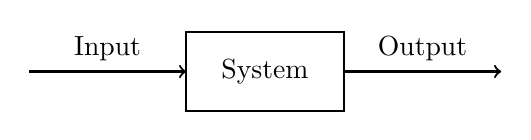
\begin{tikzpicture}
		\draw[thick, ->, color=black] (0,0) -- (2,0) node[midway, above] {Input};
		\draw[thick, color=black] (2,-0.5) rectangle (4,0.5) node[midway] {System};
		\draw[thick, ->, color=black] (4,0) -- (6,0) node[midway, above] {Output};
	\end{tikzpicture}
	\caption{Simple block diagram drawn with \texttt{tikz}.}
	\label{fig:tikz}
\end{figure}

\subsection{\texttt{pgfplots}}
The \texttt{pgfplots} package builds data plots on top of TikZ. Example of a simple function plot:

\begin{figure}[H]
	\centering
	\begin{tikzpicture}
		\begin{axis}[
			width=0.6\linewidth,
			height=5cm,
			xlabel={$x$},
			ylabel={$y$},
			grid=major,
			grid style={color=facultycolour!20}]
			\addplot[color=facultycolour, thick, domain=0:360, samples=100] {sin(x)};
		\end{axis}
	\end{tikzpicture}
	\caption{Sine wave plotted with \texttt{pgfplots}.}
	\label{fig:pgfplots}
\end{figure}

\subsection{\texttt{circuitikz}}
The \texttt{circuitikz} package draws circuit schematics. Example of a simple RC circuit:

\begin{figure}[H]
	\centering
	\begin{circuitikz}
		\draw (0,0)
		to[V, l=$V_s$] (0,2)
		to[R, l=$R$] (2,2)
		to[C, l=$C$] (2,0)
		-- (0,0);
	\end{circuitikz}
	\caption{Simple RC circuit drawn with \texttt{circuitikz}.}
	\label{fig:circuit}
\end{figure}

%%%%%%%%%%%%%%%%%%%%%%%%%%%%%%%%%%%%%%%%%%%%%%%%%%%%%%%%%%%
% ALGORITHMS
%%%%%%%%%%%%%%%%%%%%%%%%%%%%%%%%%%%%%%%%%%%%%%%%%%%%%%%%%%%
\section{Algorithms}

\subsection{\texttt{algorithm} and \texttt{algpseudocode}}
The \texttt{algorithm} package provides a float wrapper for algorithms, giving them captions, labels, and an entry in the list of algorithms. The \texttt{algpseudocode} package provides the pseudocode commands. Use \texttt{\textbackslash Require} and \texttt{\textbackslash Ensure} for inputs and outputs, and \texttt{\textbackslash Comment\{\}} for inline comments.

\begin{algorithm}[H]
	\caption{Binary Search}
	\label{alg:binarysearch}
	\begin{algorithmic}[1]
		\Require Sorted array $A$ of length $n$, search value $target$
		\Ensure Index of $target$ in $A$, or $-1$ if not found
		\Function{BinarySearch}{$A, n, target$}
		\State $low \gets 0$
		\State $high \gets n - 1$
		\While{$low \leq high$}
		\State $mid \gets \lfloor(low + high) / 2\rfloor$ \Comment{Compute midpoint}
		\If{$A[mid] = target$}
		\State \Return $mid$ \Comment{Target found}
		\ElsIf{$A[mid] < target$}
		\State $low \gets mid + 1$ \Comment{Search right half}
		\Else
		\State $high \gets mid - 1$ \Comment{Search left half}
		\EndIf
		\EndWhile
		\State \Return $-1$ \Comment{Target not found}
		\EndFunction
	\end{algorithmic}
\end{algorithm}

\begin{algorithm}[H]
	\caption{Bubble Sort}
	\label{alg:bubblesort}
	\begin{algorithmic}[1]
		\Require Array $A$ of length $n$
		\Ensure $A$ sorted in ascending order
		\Function{BubbleSort}{$A, n$}
		\For{$i \gets 0$ \textbf{to} $n - 1$}
		\For{$j \gets 0$ \textbf{to} $n - i - 2$}
		\If{$A[j] > A[j+1]$}
		\State swap $A[j]$ and $A[j+1]$ \Comment{Swap out of order elements}
		\EndIf
		\EndFor
		\EndFor
		\EndFunction
	\end{algorithmic}
\end{algorithm}

A reference to an algorithm uses \texttt{\textbackslash cref}: see \cref{alg:binarysearch} and \cref{alg:bubblesort}.

%%%%%%%%%%%%%%%%%%%%%%%%%%%%%%%%%%%%%%%%%%%%%%%%%%%%%%%%%%%
% LINKS & REFERENCES
%%%%%%%%%%%%%%%%%%%%%%%%%%%%%%%%%%%%%%%%%%%%%%%%%%%%%%%%%%%
\section{Links \& References}

\subsection{\texttt{hyperref}}
The \texttt{hyperref} package makes cross-references and URLs clickable. All links use \texttt{facultycolour}. Example URL: \url{https://www.yorku.ca}

\subsection{\texttt{cleveref}}
The \texttt{cleveref} package automatically prepends the reference type. Examples:
\begin{itemize}
	\item Equation: \cref{eq:gaussian}
	\item Figure: \cref{fig:logo}
	\item Sub-figure: \cref{fig:sub_a}
	\item Table: \cref{tab:booktabs}
	\item Algorithm: \cref{alg:binarysearch}
	\item Section: \cref{sec:lists}
	\item Theorem: \cref{thm:pythagorean}
	\item Lemma: \cref{lem:even}
	\item Proposition: \cref{prop:rational}
	\item Corollary: \cref{cor:prime}
	\item Conjecture: \cref{con:goldbach}
	\item Axiom: \cref{axm:line}
	\item Definition: \cref{def:vectorspace}
	\item Example: \cref{ex:rn}
	\item Criterion: \cref{crit:stability}
	\item Remark: \cref{rem:zerovector}
	\item Note: \cref{note:numbering}
	\item Problem: \cref{prob:ohmslaw}
\end{itemize}

%%%%%%%%%%%%%%%%%%%%%%%%%%%%%%%%%%%%%%%%%%%%%%%%%%%%%%%%%%%
% TYPOGRAPHY
%%%%%%%%%%%%%%%%%%%%%%%%%%%%%%%%%%%%%%%%%%%%%%%%%%%%%%%%%%%
\section{Typography}

\subsection{\texttt{microtype}}
The \texttt{microtype} package applies subtle typographic improvements including character protrusion and font expansion. The effect is most visible in justified text with many line breaks. It produces no visually distinct output on its own but improves overall text quality.

\subsection{\texttt{xurl}}
The \texttt{xurl} package extends \texttt{hyperref}'s URL handling by allowing line breaks at more characters, including slashes, dots, hyphens, and underscores. This prevents overfull lines when long URLs appear in the body text. URLs are colored \texttt{facultycolour} via the \texttt{\textbackslash url} command. Example: \url{https://futurestudents.yorku.ca/program/engineering-intl-development-studies}

\subsection{\texttt{indentfirst}}
The \texttt{indentfirst} package indents the first paragraph of every section, matching the behaviour of the remaining paragraphs.

This is the first paragraph of this subsection — it is indented because \texttt{indentfirst} is loaded.

This is the second paragraph — also indented as normal.

%%%%%%%%%%%%%%%%%%%%%%%%%%%%%%%%%%%%%%%%%%%%%%%%%%%%%%%%%%%
% LISTS
%%%%%%%%%%%%%%%%%%%%%%%%%%%%%%%%%%%%%%%%%%%%%%%%%%%%%%%%%%%
\section{Lists}\label{sec:lists}

\subsection{\texttt{enumitem}}
The \texttt{enumitem} package provides fine-grained control over list spacing, labels, and alignment.

Unordered list with reduced spacing:
\begin{itemize}[noitemsep]
	\item First item
	\item Second item
	\item Third item
\end{itemize}

Ordered list with custom label:
\begin{enumerate}[label=\textbf{\arabic*.}]
	\item First item
	\item Second item
	\item Third item
\end{enumerate}

Descriptive list:
\begin{description}[leftmargin=3cm, style=nextline]
	\item[\texttt{noitemsep}] Removes vertical space between items
	\item[\texttt{label}] Customises the list label format
	\item[\texttt{leftmargin}] Controls the left indent of the list
\end{description}

%%%%%%%%%%%%%%%%%%%%%%%%%%%%%%%%%%%%%%%%%%%%%%%%%%%%%%%%%%%
% PROBLEM / SOLUTION ENVIRONMENTS
%%%%%%%%%%%%%%%%%%%%%%%%%%%%%%%%%%%%%%%%%%%%%%%%%%%%%%%%%%%
\section{Problem \& Solution Environments}

\subsection{\texttt{tcolorbox}}
The \texttt{tcolorbox} package provides the \texttt{problem} and \texttt{solution} environments. Problems are automatically numbered (by section if \texttt{metaNumberProblems} is set to true).

\begin{problem}[Ohm's Law]
	\label{prob:ohmslaw}
	Given a resistor $R = \SI{10}{\ohm}$ with a voltage $V = \SI{5}{\volt}$
	across it, find the current $I$.
\end{problem}

\begin{solution}
	Applying Ohm's Law (\cref{eq:gaussian}):
	\begin{equation}
		I = \frac{V}{R} = \frac{5}{10} = \SI{0.5}{\ampere}
	\end{equation}
	\qed
\end{solution}

\begin{problem}
	\label{prob:problem}
	A problem without a title is also valid.
\end{problem}

\begin{solution}
	The optional title argument can be omitted. \qed
\end{solution}

%%%%%%%%%%%%%%%%%%%%%%%%%%%%%%%%%%%%%%%%%%%%%%%%%%%%%%%%%%%
% CODE LISTINGS
%%%%%%%%%%%%%%%%%%%%%%%%%%%%%%%%%%%%%%%%%%%%%%%%%%%%%%%%%%%
\section{Code Listings}

\subsection{\texttt{listings}}
The \texttt{listings} package provides syntax-highlighted code listings. Five styles are defined: \texttt{matlab}, \texttt{java}, \texttt{python}, \texttt{cpp}, and \texttt{latex}.

\subsubsection{MATLAB}
\begin{lstlisting}[style=matlab]
	x = 0:0.1:2*pi;
	y = sin(x);
	plot(x, y);
	xlabel('x'); ylabel('sin(x)');
	title('Sine Wave');
\end{lstlisting}

\subsubsection{Java}
\begin{lstlisting}[style=java]
	public class HelloWorld {
		public static void main(String[] args) {
			System.out.println("Hello, World!");
		}
	}
\end{lstlisting}

\subsubsection{Python}
\begin{lstlisting}[style=python]
	import numpy as np
	import matplotlib.pyplot as plt
	
	x = np.linspace(0, 2 * np.pi, 100)
	y = np.sin(x)
	plt.plot(x, y)
	plt.show()
\end{lstlisting}

\subsubsection{C++}
\begin{lstlisting}[style=cpp]
	#include <iostream>
	using namespace std;
	
	int main() {
		cout << "Hello, World!" << endl;
		return 0;
	}
\end{lstlisting}

\subsubsection{\LaTeX}
\begin{lstlisting}[style=latex]
	\begin{equation}
		E = mc^2
		\label{eq:einstein}
	\end{equation}
	See \cref{eq:einstein} for Einstein's mass-energy equivalence.
\end{lstlisting}

%%%%%%%%%%%%%%%%%%%%%%%%%%%%%%%%%%%%%%%%%%%%%%%%%%%%%%%%%%%
% DRAFT TOOLS
%%%%%%%%%%%%%%%%%%%%%%%%%%%%%%%%%%%%%%%%%%%%%%%%%%%%%%%%%%%
\section{Draft Tools}

\subsection{\texttt{todonotes}}
\todo{This is a margin to do note.}
The \texttt{todonotes} package adds margin and inline notes. Controlled by \texttt{\textbackslash metaShowTodo} in the metadata.

\todo[inline]{This is an inline to do note.}

\subsection{\texttt{draftwatermark}}
The \texttt{draftwatermark} package overlays a diagonal watermark. Set \texttt{\textbackslash metaWatermarkText} in the metadata to enable it. It is currently \ifthenelse{\equal{\metaWatermarkText}{}}{disabled}{enabled}.

\subsection{\texttt{lipsum}}
The \texttt{lipsum} package generates dummy text for testing layout:

\lipsum[1]

%%%%%%%%%%%%%%%%%%%%%%%%%%%%%%%%%%%%%%%%%%%%%%%%%%%%%%%%%%%
% HEADER & FOOTER
%%%%%%%%%%%%%%%%%%%%%%%%%%%%%%%%%%%%%%%%%%%%%%%%%%%%%%%%%%%
\section{Header \& Footer}

\subsection{\texttt{fancyhdr}}
The \texttt{fancyhdr} package provides custom headers and footers. This template uses it to display the course code and name on the left, the student name on the right, and the page number centred in the footer, on all pages after the title page. The header rule is rendered in \texttt{facultycolour}. It produces no additional visible output here beyond what is already visible at the top and bottom of every page.

%%%%%%%%%%%%%%%%%%%%%%%%%%%%%%%%%%%%%%%%%%%%%%%%%%%%%%%%%%%
% BIBLIOGRAPHY
%%%%%%%%%%%%%%%%%%%%%%%%%%%%%%%%%%%%%%%%%%%%%%%%%%%%%%%%%%%
\section{Bibliography}

\subsection{\texttt{csquotes}}
The \texttt{csquotes} package provides context-sensitive quotation marks and is required by \texttt{biblatex}. It produces no visible output on its own.

\subsection{\texttt{biblatex}}
The \texttt{biblatex} package handles citations and bibliography generation using Biber as the backend. The citation style is controlled by \texttt{\textbackslash metaBibStyle} in the metadata (\texttt{ieee} or \texttt{apa}). The current style is \texttt{\metaBibStyle}. Add entries to your \texttt{.bib} file and cite them with \texttt{\textbackslash cite\{\}}. Example citation: \cite{example}.

%%%%%%%%%%%%%%%%%%%%%%%%%%%%%%%%%%%%%%%%%%%%%%%%%%%%%%%%%%%
% REFERENCES
%%%%%%%%%%%%%%%%%%%%%%%%%%%%%%%%%%%%%%%%%%%%%%%%%%%%%%%%%%%
\newpage
\phantomsection % Allows TOC to link to references
\printbibliography[heading=bibintoc] % Need square bracket content for TOC

%%%%%%%%%%%%%%%%%%%%%%%%%%%%%%%%%%%%%%%%%%%%%%%%%%%%%%%%%%%
% APPENDICES
%%%%%%%%%%%%%%%%%%%%%%%%%%%%%%%%%%%%%%%%%%%%%%%%%%%%%%%%%%%
\newpage
\appendix % Insert this and all below to create appendix
\titleformat{\section}
{\Large\bfseries\color{facultycolour}}
{Appendix~\Alph{section}}
{1em}{}
\renewcommand{\thesection}{\Alph{section}}
\renewcommand{\thefigure}{\Alph{section}.\arabic{figure}}
\renewcommand{\thetable}{\Alph{section}.\arabic{table}}
\renewcommand{\theequation}{\Alph{section}.\arabic{equation}}
\renewcommand{\theproblem}{\Alph{section}.\arabic{problem}}
\renewcommand{\thetheorem}{\Alph{section}.\arabic{theorem}}
\renewcommand{\thealgorithm}{\Alph{section}.\arabic{algorithm}}
\counterwithin{figure}{section}
\counterwithin{table}{section}
\counterwithin{equation}{section}
\counterwithin{problem}{section}
\counterwithin{theorem}{section}
\counterwithin{algorithm}{section}

\section{Supplementary Data}\label{sec:appendix-supp}

This appendix demonstrates how appendix sections are formatted. Section headings are
relabelled as \textbf{Appendix A}, \textbf{Appendix B}, etc., and figures, tables,
and equations are prefixed with the corresponding letter.

\begin{table}[H]
	\centering
	\caption{Sample supplementary data table.}
	\label{tab:appendix_data}
	\begin{tabular}{@{}lcc@{}}
		\toprule
		Parameter & Measured & Unit \\
		\midrule
		Temperature & 23.4 & \si{\celsius} \\
		Pressure    & 101.3 & \si{\kilo\pascal} \\
		Humidity    & 48.7 & \% \\
		\bottomrule
	\end{tabular}
\end{table}

\begin{figure}[H]
	\centering
	\begin{tikzpicture}
		\begin{axis}[
			width=0.6\linewidth,
			height=5cm,
			xlabel={Time (\si{\second})},
			ylabel={Amplitude},
			grid=major,
			grid style={color=facultycolour!20}]
			\addplot[color=facultycolour, thick, domain=0:360, samples=100] {cos(x)};
		\end{axis}
	\end{tikzpicture}
	\caption{Sample cosine plot included as supplementary material.}
	\label{fig:appendix_plot}
\end{figure}

To attach an external PDF (e.g.\ a datasheet), replace the content above with:
\begin{lstlisting}[style=latex]
	\includepdf[pages=-]{filename.pdf}
\end{lstlisting}

\newpage
\section{Notation}

This appendix lists the mathematical notation used throughout the document.

\begin{table}[H]
	\centering
	\caption{Summary of notation.}
	\label{tab:notation}
	\begin{tabularx}{\linewidth}{@{}lX@{}}
		\toprule
		Symbol & Meaning \\
		\midrule
		$\bm{F}$ 	 & Force vector (\si{\newton}) \\
		$m$      & Mass (\si{\kilo\gram}) \\
		$\bm{a}$ 	 & Acceleration vector (\si{\metre\per\second\squared}) \\
		$V$      & Voltage (\si{\volt}) \\
		$I$      & Current (\si{\ampere}) \\
		$R$      & Resistance (\si{\ohm}) \\
		\bottomrule
	\end{tabularx}
\end{table}
